\chapter{$M_{\rm BH} - n_{\rm sph}$}
\label{ch:mn}

While the previous Chapter was dedicated to the study of the relations between 
black hole mass and galaxy or spheroid luminosity, 
in this Chapter we will perform an analogous analysis 
to explore the relation between black hole mass and spheroid S\'ersic index ($M_{\rm BH} - n_{\rm sph}$). 
To address the issue of consistency between galaxy scaling relations 
that was outlined in Chapter \ref{ch:intro}, 
it is mandatory to include also an analysis of the relation between spheroid luminosity 
and spheroid S\'ersic index ($L_{\rm sph} - n_{\rm sph}$). 
The reliability of the uncertainties associated with the S\'ersic index measurements 
obtained from our 1D decompositions 
ensures a robust estimate of the intrinsic scatter in the $M_{\rm BH} - n_{\rm sph}$ diagram, 
which can be compared with that in the $M_{\rm BH} - L_{\rm sph}$ diagram. \\

The remainder of this chapter comprises the peer-reviewed version of the paper 
``Supermassive Black Holes and Their Host Spheroids. 
III. The $M_{\rm BH} - n_{\rm sph}$ correlation'' 
by G.~A.~D.~Savorgnan,  
accepted for publication in the \emph{The Astrophysical Journal}. 



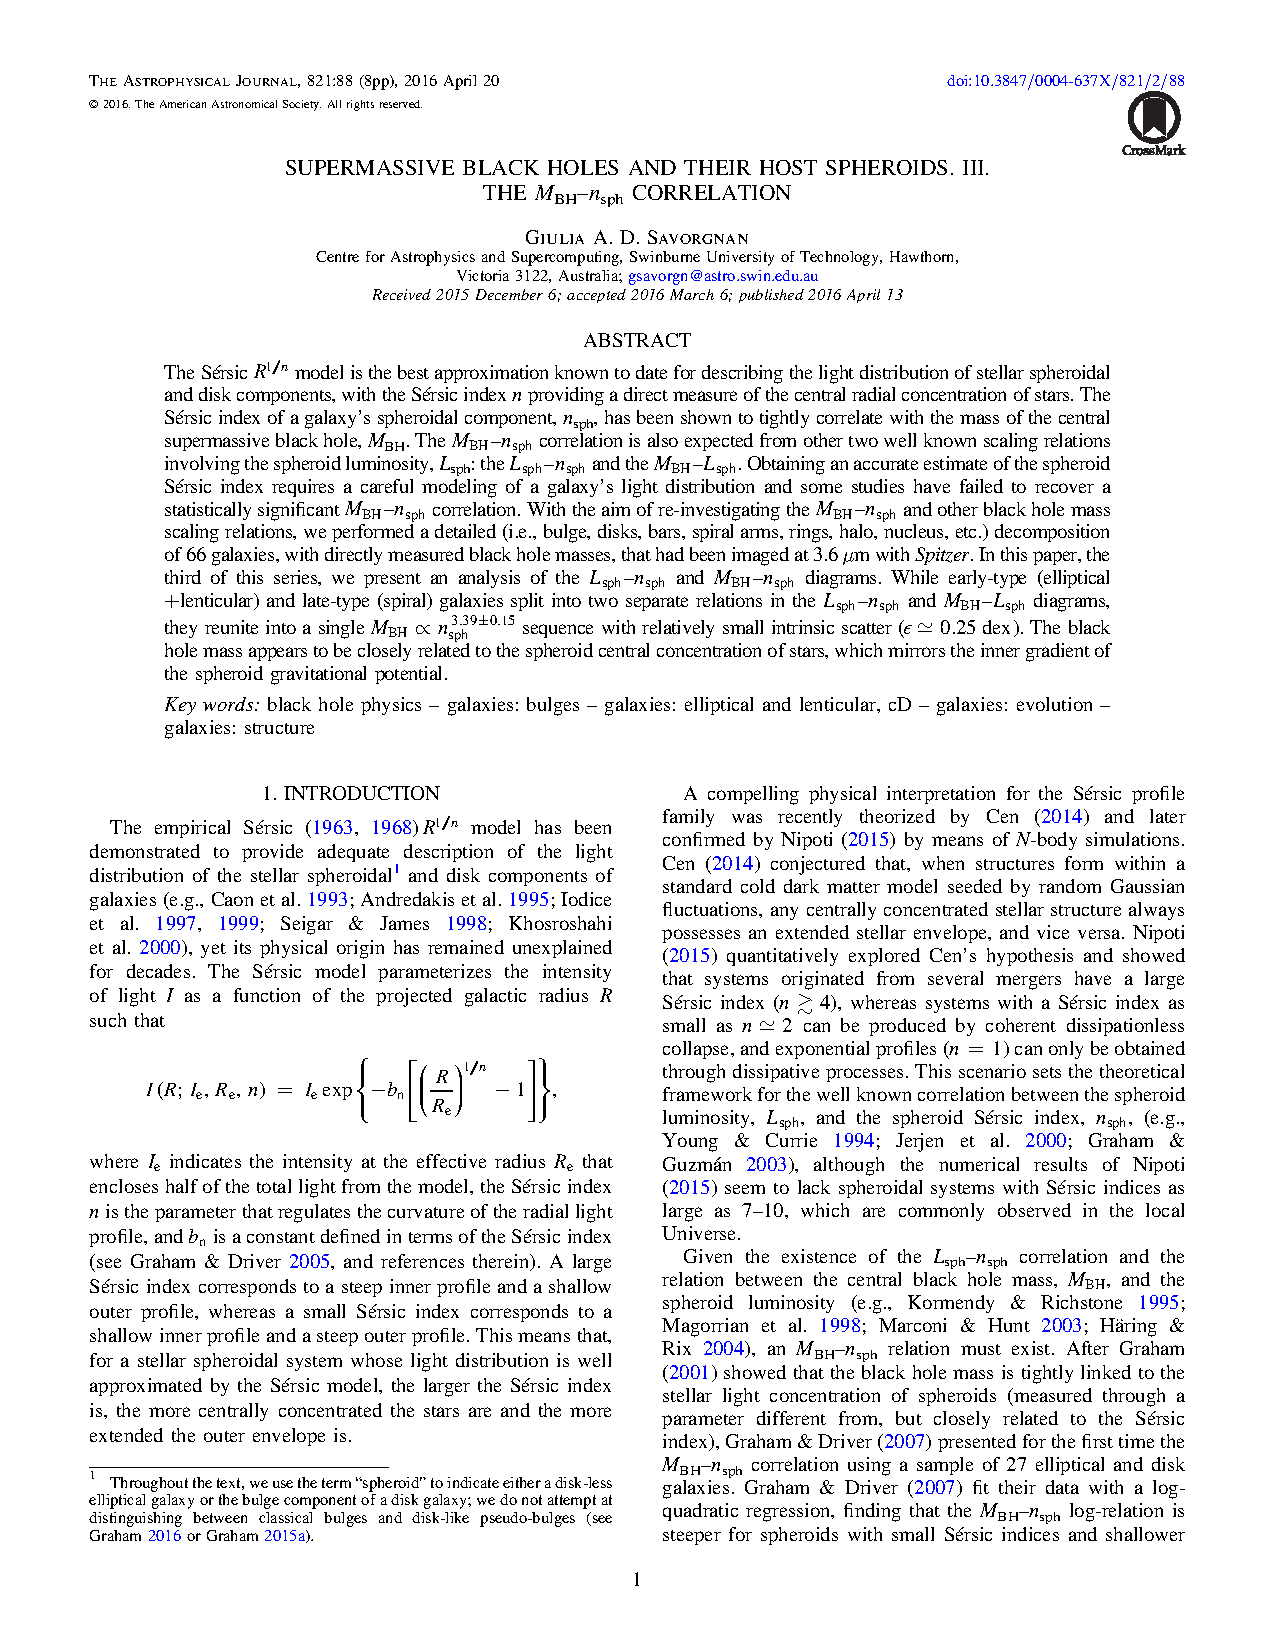
\includepdf[pages={1-10}]{ApJ2016b.pdf}
